\section*{Exercise 7 Simulated annealing(Comments by Qahir)}
As the jumping set we permute two random stations on the route and hence the jumping distribution is symmetric. On figure \ref{fig:ex7} pseudo-code for the simulated annealing can be seen. We let $V$ denote our energy function. 

\begin{figure}[H]
    \hrule
    \vspace*{0.2cm}
    \begin{enumerate}
    \item Initialize $X$ as random permutations of $\{0,1,...,n-1\}$ and $i=0$. 
    \item Set $X^* \leftarrow X$ and $V^* \leftarrow V(X^*)$
    \item Generate proposal $Y$ by interchanging two elements of $X$
    \item Set $R = \exp(-\frac{V(Y)-V(X)}{T(i)})$
    \item If $R > 1$ set $X \leftarrow Y$
    \item Else set $X \leftarrow Y$ with probability $R$
    \item If $V(X) < V(X^*)$ set $X^* \leftarrow X$, $V^* \leftarrow V(X)$
    \item Repeat steps (3)-(8) for $i = 1,...,N_{samples}-1$. 
    \end{enumerate}
    \vspace*{0.2cm}
    \hrule
    \vspace*{0.2cm}
    \caption{Pseudo-code for Simulated annealing.}
    \label{fig:ex7}
\end{figure}

The code was verified by testing on the travelling salesman problem for $10$ points spread equidistantly on the unit circle. Here the cooling scheme was set such that $T_k = \frac{1}{\sqrt{1+k}}$. Here $500$K samples were run. Along with this $2000$K samples for the cost matrix function from the course homepage here the cost was found to be $1163$. It is seen that the code is capable of solving the problem for the $10$ equidistant points on the unit circle. For the problem with the cost matrix function from the course homepage we are probably stuck at a local minima. This can be verified by running the sampler multiple times and here we end up with costs ranging from $1100-1300$. Picking cooling scheme that does not go to zero as quickly when $i \rightarrow \infty$ would probably be a good idea. Trying with the one provided in the notes - $T_k = \frac{1}{\text{log(1+k)}}$ does not provide a better result. The code can be found in the appendix. 
\begin{figure}[H]
        \centering
        \begin{subfigure}[H]{0.475\textwidth}
            \centering
            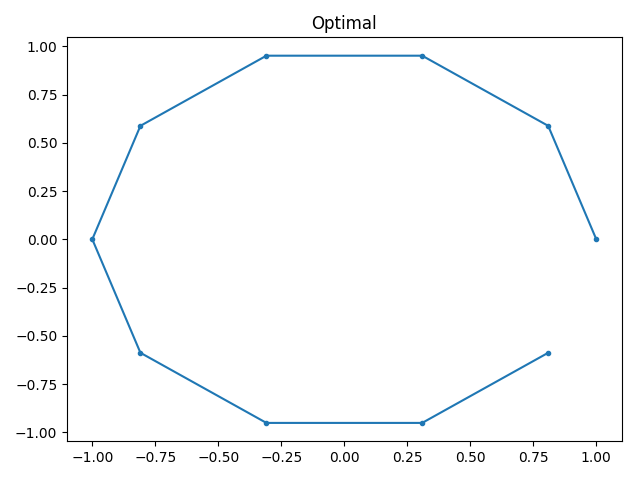
\includegraphics[width=\textwidth]{figures/optimal.png}
            \caption[Network2]%
            {{\small Optimal for $10$ equidistant points of the unit circle.}}    
            \label{fig:Star4}
        \end{subfigure}
        \hfill
        \begin{subfigure}[H]{0.475\textwidth}  
            \centering 
            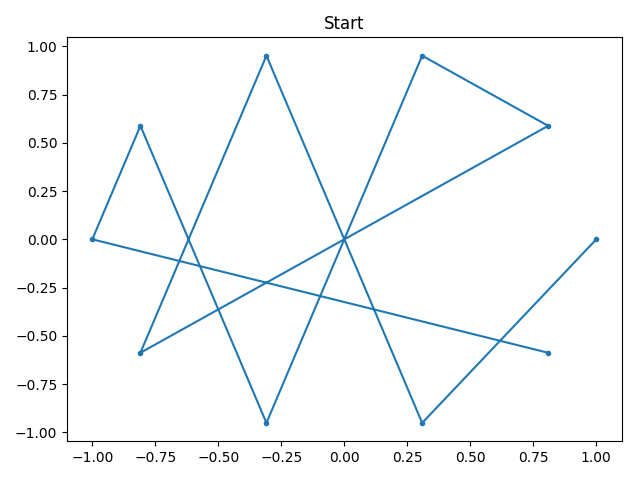
\includegraphics[width=\textwidth]{figures/start.png}
            \caption[]%
            {{\small Initial permutation for $10$ equidistant points of the unit circle.}}    
            \label{fig:mean and std of net24}
        \end{subfigure}
        \vskip\baselineskip
        \begin{subfigure}[H]{0.475\textwidth}   
            \centering 
            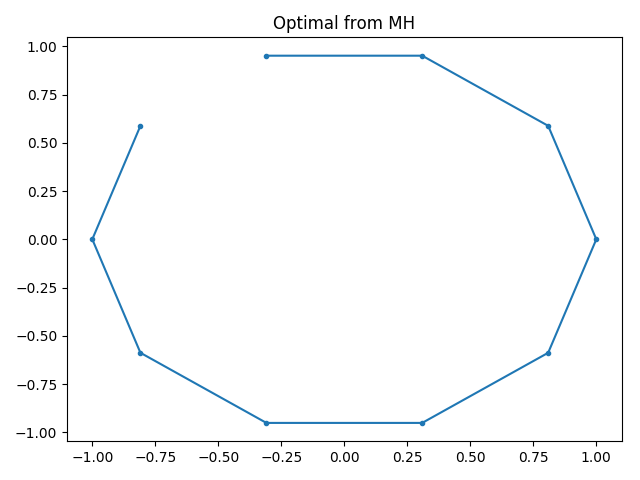
\includegraphics[width=\textwidth]{figures/mh.png}
            \caption[]%
            {{\small Simulated annealing solution for $10$ equidistant points on the unit circle.}}    
            \label{fig:mean and std of net34}
        \end{subfigure}
        \quad
        \begin{subfigure}[H]{0.475\textwidth}   
            \centering 
            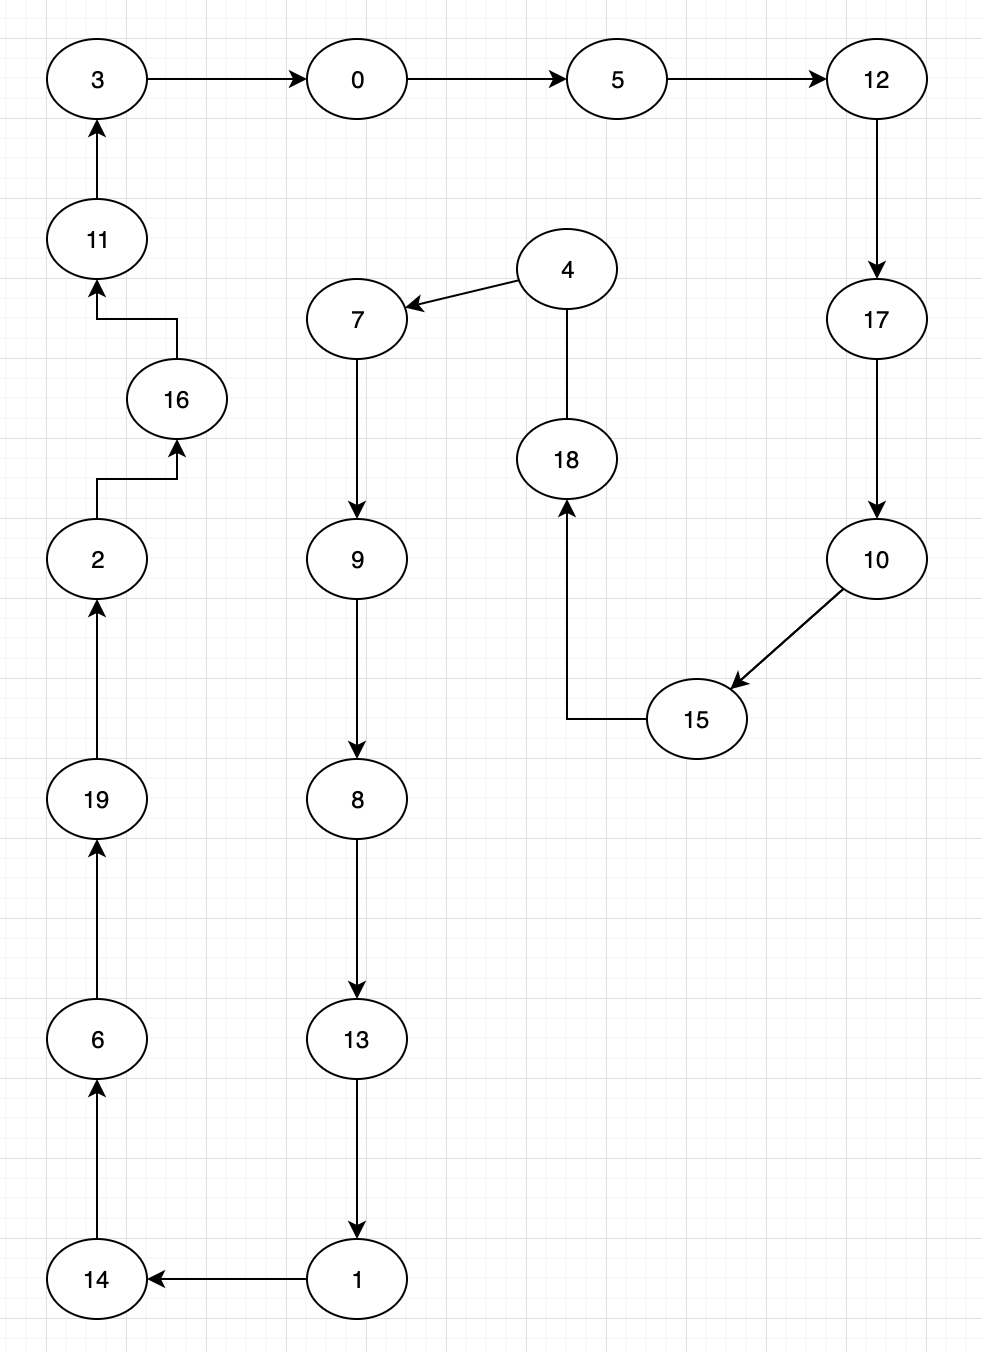
\includegraphics[width=\textwidth]{figures/matrix.png}
            \caption[]%
            {{\small Diagram of optimal permutation for cost matrix problem.}}    
            \label{fig:stuff}
        \end{subfigure}
        \caption[ The average and standard deviation of critical parameters ]
        {\small $20000$ Simulated anealing figures } 
        \label{fig:ex71}
    \end{figure}

\textbf{Comments by Sen}

In the simulated annealing part, two exercises have been done, with one being a test for the scheme and another one being the classical travelling salesman problem. The general scheme is the same as in figure \ref{fig:ex7}. New route is created by randomly switching two stations. Temperature is decreased with increasing iterations with $T_{k}=1 / \sqrt{1+k}$. For the test case, the algorithm successfully reaches the optimal route as shown in figure \ref{fig:debugsen}.
\begin{figure}[H]
    \centering
    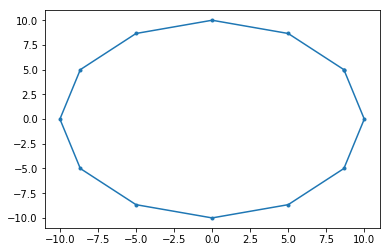
\includegraphics{figures/debugsen.png}
    \caption{Result for debug process}
    \label{fig:debugsen}
\end{figure}

\begin{figure}[H]
    \centering
    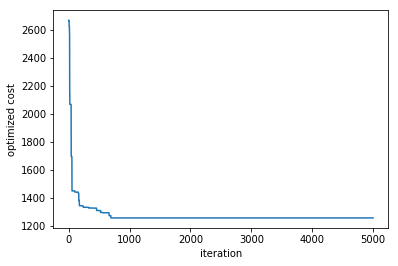
\includegraphics{figures/annealing.png}
    \caption{Optimized cost vs. iterations}
    \label{fig:annellingSen}
\end{figure}

For the given case, a final cost of 1256 is obtained. The route is 15, 10, 2, 19, 5, 11, 18, 14, 8, 13, 1, 6, 17, 16, 0, 12, 3, 7, 4, 9, 15. Figure \ref{fig:annellingSen} depicts the best route with progressing iterations. After around 700 iterations, the cost drops to 1256 and keeps stable afterwards, which should be a local minimum. Besides from keep running the algorithm, possible ideas can be proposed in order for jumping out of the local minimum. For example, increase the temperature or use a new scheme to generate new route (e.g. switch 3 stations) when there is no change after 1000 consecutive iterations. 

